\documentclass[10pt]{article}
\usepackage{amssymb}
\usepackage{pgf,tikz}
\usetikzlibrary{arrows, fit, shapes, arrows.meta, snakes,
positioning, matrix}
\usepackage{tkz-graph}
\pgfdeclarelayer{bg}
\pgfsetlayers{bg,main}

\begin{document}

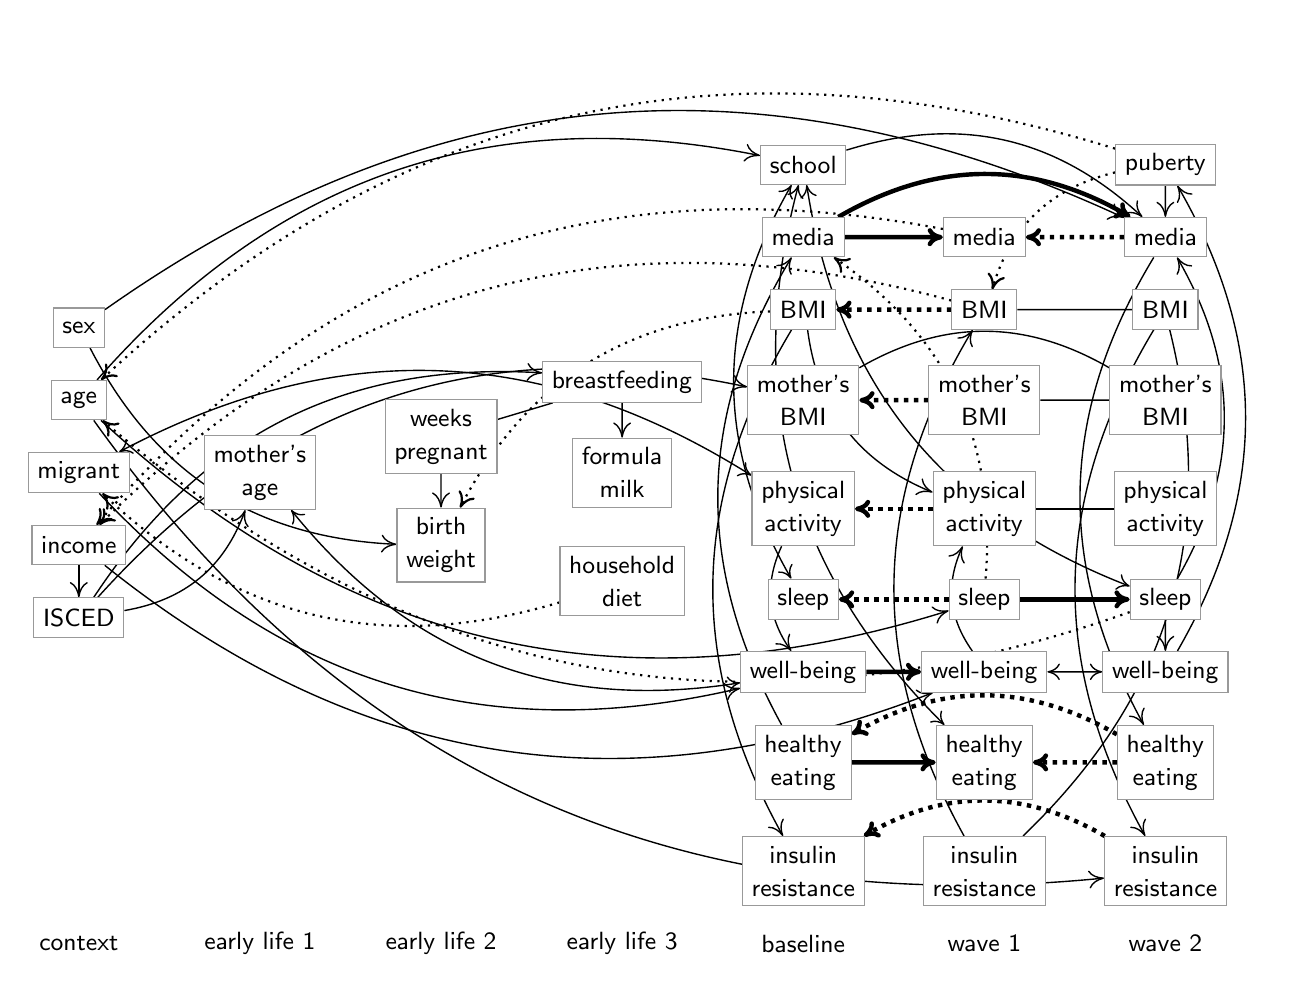
\begin{tikzpicture}[scale=0.92, squarednode/.style={rectangle, draw=gray!80, fill=white, thin, minimum size=5mm}]

\node[squarednode] (sex) at (0, 2.75) {\small \textsf{sex}};
\node[squarednode] (age) at (0, 1.75) {\small \textsf{age}};
\node[squarednode] (migrant) at (0, 0.75) {\small  \textsf{migrant}};
\node[squarednode] (income) at (0, -.25) {\small \textsf{income}};
\node[squarednode] (isced) at (0,-1.25) {\small \textsf{ISCED}};

\node[squarednode, align=center] (bage) at (2.5,0.75) {\small \textsf{mother's} \\ \small \textsf{age}};

\node[squarednode, align=center] (pregweek) at (5, 1.25) {\small \textsf{weeks} \\ \small \textsf{pregnant}};
\node[squarednode, align=center] (bweight) at (5, -.25) {\small \textsf{birth} \\ \small \textsf{weight}};

\node[squarednode] (bf) at (7.5, 2) {\small \textsf{breastfeeding}};
\node[squarednode, align=center] (formula) at (7.5, 0.75) {\small \textsf{formula}\\ \small \textsf{milk}};
\node[squarednode, align=center] (hdiet) at (7.5, -.75) {\small \textsf{household}\\ \small \textsf{diet}};

\node[squarednode] (school) at (10,5) {\small \textsf{school}};
\node[squarednode] (media0) at (10,4) {\small \textsf{media}};
\node[squarednode] (bmi0) at (10, 3) {\small \textsf{BMI}};
\node[squarednode, align=center] (mbmi0) at (10, 1.75) {\small \textsf{mother's}\\ \small \textsf{BMI}};
\node[squarednode, align=center] (pa0) at (10, 0.25) {\small \textsf{physical}\\ \small \textsf{activity}};
\node[squarednode] (sleep0) at (10, -1) {\small \textsf{sleep}};
\node[squarednode] (wb0) at (10, -2) {\small \textsf{well-being}};
\node[squarednode, align=center] (yhei0) at (10, -3.25) {\small \textsf{healthy}\\ \small \textsf{eating}};
\node[squarednode, align=center] (homa0) at (10, -4.75) {\small \textsf{insulin}\\\small \textsf{resistance}};

\node[squarednode] (media1) at (12.5,4) {\small \textsf{media}};
\node[squarednode] (bmi1) at (12.5, 3) {\small \textsf{BMI}};
\node[squarednode, align=center] (mbmi1) at (12.5, 1.75) {\small \textsf{mother's}\\ \small \textsf{BMI}};
\node[squarednode, align=center] (pa1) at (12.5, 0.25) {\small \textsf{physical}\\ \small \textsf{activity}};
\node[squarednode] (sleep1) at (12.5, -1) {\small \textsf{sleep}};
\node[squarednode] (wb1) at (12.5, -2) {\small \textsf{well-being}};
\node[squarednode, align=center] (yhei1) at (12.5, -3.25) {\small \textsf{healthy}\\ \small \textsf{eating}};
\node[squarednode, align=center] (homa1) at (12.5, -4.75) {\small \textsf{insulin}\\\small \textsf{resistance}};

\node[squarednode] (pub) at (15, 5) {\small \textsf{puberty}};
\node[squarednode] (media2) at (15,4) {\small \textsf{media}};
\node[squarednode] (bmi2) at (15, 3) {\small \textsf{BMI}};
\node[squarednode, align=center] (mbmi2) at (15, 1.75) {\small \textsf{mother's}\\ \small \textsf{BMI}};
\node[squarednode, align=center] (pa2) at (15, 0.25) {\small \textsf{physical}\\ \small \textsf{activity}};
\node[squarednode] (sleep2) at (15, -1) {\small \textsf{sleep}};
\node[squarednode] (wb2) at (15, -2) {\small \textsf{well-being}};
\node[squarednode, align=center] (yhei2) at (15, -3.25) {\small \textsf{healthy}\\ \small \textsf{eating}};
\node[squarednode, align=center] (homa2) at (15, -4.75) {\small \textsf{insulin}\\\small \textsf{resistance}};

\tikzset{undir/.style = {-, line width = 0.5pt}}
\tikzset{dir/.style = {->, -{To[length=5.5, width=6.5]}, line width = 0.5pt}}
\tikzset{bidir/.style = {{To[length=4.5, width=6]}-{To[length=4.5, width=6]}, line width = 0.5pt}}

\node (t1) at (0, -5.75) {\small \textsf{context}};
\node (t2) at (2.5, -5.75) {\small \textsf{early life 1}};
\node (t3) at (5, -5.75) {\small \textsf{early life 2}};
\node (t4) at (7.5, -5.75) {\small \textsf{early life 3}};
\node (t5) at (10, -5.75) {\small \textsf{baseline}};
\node (t6) at (12.5, -5.75) {\small \textsf{wave 1}};
\node (t7) at (15, -5.75) {\small \textsf{wave 2}};


 \begin{pgfonlayer}{bg}
\draw[undir]
(pregweek) edge  (bf)
(mbmi0) edge [bend left] (mbmi2)
(mbmi1) edge (mbmi2)
(bmi1) edge (bmi2)
(pa1) edge (pa2)
(homa1) edge [bend right] (bmi2) 
;

\draw[bidir]
(migrant) edge [bend left] (pa0)
(bage) edge [bend right] (wb0)
(school) edge [bend right] (sleep0)
(school) edge [bend right] (yhei1)
(school) edge [bend right] (sleep2)
(wb1) edge (wb2)
;

\draw[dir]
(sex) edge [bend right] (bweight)
(sex) edge [bend left] (media2)
(age) edge [bend left] (school)
(age) edge [bend right] (sleep1)
(age) edge [bend right] (homa2)
(migrant) edge [bend right] (wb0)
(income) edge (isced)
(income) edge [bend right] (wb1)
(isced) edge [bend right] (bage)
(isced) edge [bend left] (bf)
(isced) edge [bend left] (mbmi0)
(pregweek) edge (bweight)
(bf) edge (formula)
(hdiet) edge [bend left, dotted, thick] (migrant)
(school) edge [bend left] (media2)
(media0) edge [ultra thick] (media1)
(media0) edge [bend left, ultra thick] (media2)
(bmi0) edge [bend right, dotted, thick] (bweight)
(bmi0) edge [bend right] (homa0)
(bmi0) edge [bend right] (pa1)
(pa0) edge [bend right] (wb0)
(wb0) edge [ultra thick] (wb1)
(yhei0) edge [bend left] (media0)
(yhei0) edge [ultra thick] (yhei1)
(media1) edge [bend right, thick, dotted] (income)
(bmi1) edge [bend right, thick, dotted] (income)
(bmi1) edge [ultra thick, dotted] (bmi0)
(mbmi1) edge [ultra thick, dotted] (mbmi0)
(pa1) edge [ultra thick, dotted] (pa0)
(sleep1) edge [thick, dotted, bend right] (media0)
(sleep1) edge [ultra thick, dotted] (sleep0)
(sleep1) edge [ultra thick] (sleep2)
(wb1) edge [bend left] (pa1)
(homa1) edge [bend left] (bmi1)
(media2) edge [ultra thick, dotted] (media1)
(media2) edge [bend right] (yhei2)
(bmi2) edge [bend right] (homa2)
(pub) edge [bend right, thick, dotted] (age)
(pub) edge [bend right, thick, dotted] (bmi1)
(pub) edge (media2)
(sleep2) edge [bend left, thick, dotted] (age)
(sleep2) edge [bend right] (media2)
(sleep2) edge (wb2)
(wb2) edge [bend right] (pub)
(yhei2) edge [bend right, ultra thick, dotted] (yhei0)
(yhei2) edge [ultra thick, dotted] (yhei1)
(homa2) edge [bend right, ultra thick, dotted] (homa0)
;
\end{pgfonlayer}
\end{tikzpicture}

\end{document}